In our system there are four main layers, which are classified as web interface layer, wireless connection layer, base station layer, camera layer. The user can communicate with the remote surveillance camera with the help of the user interface. The Ethernet and black box will bridge between the user and the remote camera. User interface will include all kinds of resources that user is capable of using. In the system streaming video is made available and some of the controls that user can use through his computer. In the camera layer we have our camera module, which can be rotated and tilted 180 degrees, which makes it 360- degree total movement possible. In the network layer we will be using Ethernet connection. The source of the power for the camera layer and black box is base station. The main power source for the base station is solar battery.


\begin{figure}[h!]
	\centering
 	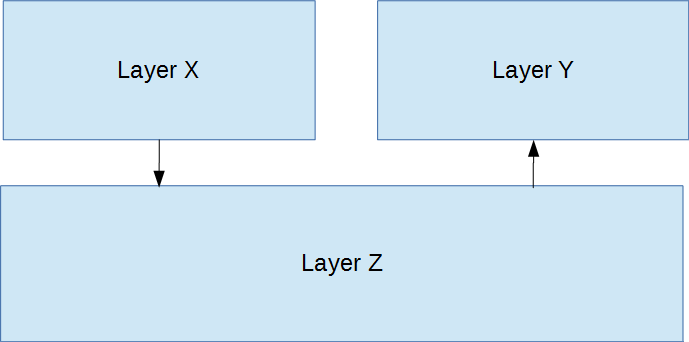
\includegraphics[width=0.60\textwidth]{images/layers}
 \caption{A simple architectural layer diagram}
\end{figure}

\subsection{Layer Web Interface Description}
The web interface layer provides high level interface for the user to communicate with the hardware or camera layer. Our system is going to have login, feedback and arrow keys. User will simply have to login for the security purpose. Each and every camera will have its unique IP, which will provide identity to the camera. For time being the username and the password will be saved in the raspberry pi, which is integrated in the camera. Feedback means the live streaming video or image captured by the camera. There are arrow keys buttons, which will help user to control the functions of the camera. Functions of the camera includes rotating and tilting camera, which is 180-degree rotation and 180-degree tilt. The movement of the camera is 360-degree total including rotation and tilting.


\subsection{Layer Camera Description}
Camera layer will provide user with high level interface layer to communicate and control hardware devices. This layer includes camera module, stepper motors, lens, raspberry pi, stepper motor driver and database. The Ethernet connection connected with raspberry pi is working as the medium to connect raspberry pi with the black box. ZeroMQ library has been installed in raspberry pi, which helps receive and send messages back and forth. Two stepper motors have been integrated, whose movement is controlled by the stepper motor drivers. The stepper motor driver has been installed in the raspberry pi. Lens is integrated with the camera module, which is tilted and rotated by the stepper motors. For time being our system is going to have a database that will save the username and password in the raspberry pi. This is the only layer of security we have it in our system, which will prevent unauthorized access.




\subsection{Layer Z Description}
Each layer should be described separately in detail. Descriptions should include the features, functions, critical interfaces and interactions of the layer. The description should clearly define the services that the layer provides. Also include any conventions that your team will use in describing the structure: naming conventions for layers, subsystems, modules, and data flows; interface specifications; how layers and subsystems are defined; etc. 
